In this section we will go through which design considerations we had when making the game.\

\subsection{Game Features}
The game prototype we created has the following features:

\begin{enumerate}
	\item iOS Mobile Application
	\item Text story
	\item Events with player choice
	\item Event and character pictures with simple animations and sounds
	\item Map, where you can select where to go (Only on place to choose from in the prototype)
	\item Battle system where dogs battle eachother
	\item Ability to train dogs
	\item Ability to catch dogs (Will never succeed in the prototype)
	\item Option to breed dogs (Will never succeed in the prototype)
\end{enumerate}

\begin{figure}[h!] 
	\centering
    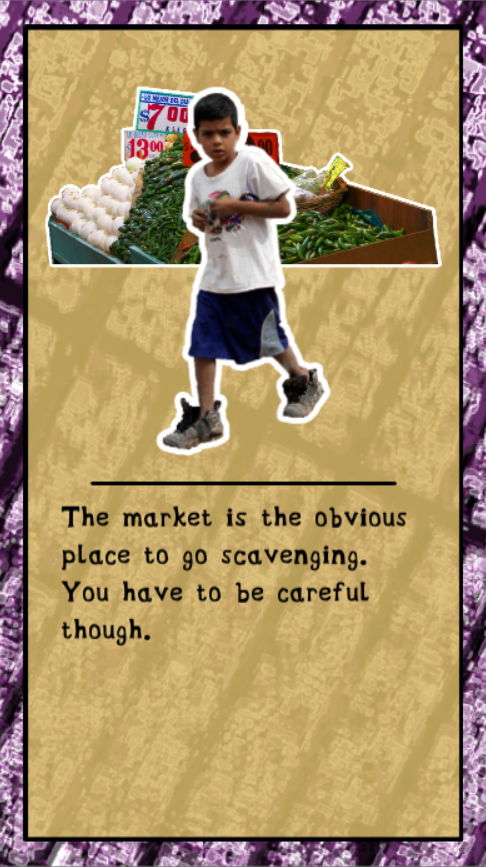
\includegraphics[width=0.5\textwidth]{GameScreen1.png}
    \caption{Story screen from the \textit{Rat Kid Dog Fight!} prototype}
    \label{fig:GameScreen}
\end{figure}

%why did we choose which features?

We chose a vertical (instead of horizontal) display for the phone for accessibility and to signal the briefness of the play session.

\subsection{Covering Prototype Limitations}
\label{limitations}
While we were creating a limited and deterministic prototype, we made several considerations, to hide the procedural and deterministic nature of the prototype. These include the map system, the ability to catch and breed, which all speak to a bigger game than the prototype is. The reason for doing this was to create an illusion of a longer game, and a potentially longer relationship with the dog. We feared that if the player knew the scale of the prototype or the already determined outcomes, they would not allow themselves to become emotionally attached to the dog. \

To create this illusion the UI is not build for simply supporting the features of the prototype, but also to support the affordances a longer and less procedural game could include. The option to 'Breed' the dogs is a feature that is not actually included in the prototype, but since the player is forced to only catch dogs of one specific gender, they will never discover this.\

\subsection{Lack of Player Agency in Fights}
As mentioned in \ref{Agency} we have implemented impotent options in the dog fights, which aims to create the illusion of agency. These options mimic the \textit{Pokémon} games, as seen in figure \ref{fig:PokeBattle} and \ref{fig:DogFightBattle}. \

\begin{figure}[h!] 
	\centering
    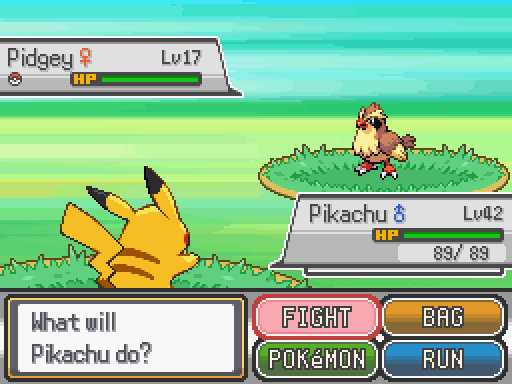
\includegraphics[width=0.5\textwidth]{PokemonBattle.png}
    \caption{A \textit{Pokémon} battle}
    \label{fig:PokeBattle}
\end{figure}

\begin{figure}[h!]
	\centering
    \includegraphics[width=0.5\textwidth]{battle.png}
    \caption{A \textit{Rat Kid Dog Fight!} battle}
    \label{fig:DogFightBattle}
\end{figure}

All these battle options does not have any effect on the actual battle. The \textit{Fight} option let the player select between \textit{Throat Bite}, \textit{Tackle}, \textit{Scratch} and \textit{Lock Bite}. While \textit{Scratch} and \textit{Tackle} are typical generic \textit{Pokémon} moves, the other two also resemble names of moves from \textit{Pokémon} with a dog fight connotation, which also makes them appear more visceral and brutal. When chosen, all of these fight-options simply give the text feedback of your character shouting something appropiate, like "Go for the throat, DOGNAME!" for selecting \textit{Throat Bite}, which also is a mediation of the television series \textit{Pokémon: The Series} (1997), where the main character, \textit{Ash}, could shout "Pikachu, use Thunderbolt!". This reference further creates the expectance of an actual effect on gameplay, since those familiar with the show, would know that there is always a direct link between what the Pokémon trainer shouts and what the Pokémon does and would expect the same causality here.
The option \textit{item} simply states that the player has no items to use and then progresses the battle. Likewise, the option \textit{Dog} states that the player "... cannot change dogs during this fight.". Similar to the (lacking) features mentioned in \ref{limitations}, this gives the player an idea of a bigger game, where they might unlock these options later on.\

The goal with creating this illusion of player agency is to create a feeling of helplessness and hopefully the realization of no agency will put them in the place of the kid. 
\commenting{ref to 'Papers, Please'}
We want to battles to be realistically random\commenting{different word} and brutal, while still giving the player the illusion of being able to change the inevitable, creating the same superstition as mentioned in \ref{Agency}.\

\subsection{Battle System}
\label{battleSystem}
Even though the player has limited agency in the fight system, we still simulate the fights with a very game-like system.\

\begin{figure}[h!]
	\centering
    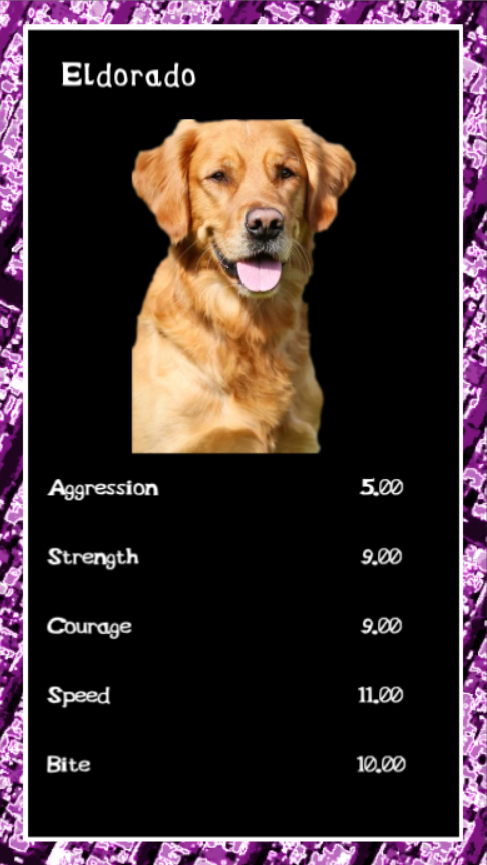
\includegraphics[width=0.5\textwidth]{DogStats.png}
    \caption{A dog stat screen from the \textit{Rat Kid Dog Fight!} prototype}
    \label{fig:DogStatScreen}
\end{figure}


The dogs has the following 5 stats: \textit{Aggression}, \textit{Strength}, \textit{Courage}, \textit{Speed} and \textit{Bite}.\

The battle system works in the following way:

\begin{center}
\scriptsize 
	\begin{tabular}{|l|p{5cm}|p{3cm}|p{3cm}|} 
		\hline
		\textbf{Game Round} & \textbf{Description} & \textbf{Example Outcome} &\textbf{ Feedback }\\ [0.5ex] 
		\hline\hline
		Aggression Roll & Each dog has a an aggression score. The one with the highest aggression will decrease the other dogs strength speed and bite depending on the others courage rating & Dog1s 10 AGGRESSION goes against Dog2s 6 courage and decreases Dog2s STRENGTH, SPEED and BITE by 40\% & "Dog2 is intimidated by the vicious barking from Dog1" \\  
		\hline\hline
		\textit{\textbf{Main loop}} \\
		\hline
		Speed Roll	& The dog with the highest roll, determined by speed bites first. &	Dog1 bites first & "Dog1 snaps after Dog2s neck. \\
		\hline
		Bite roll & The biting dogs rolls BITE against STRENGTH to penetrate to kill or injur the other dog. Max roll will always penetrate, Penetrating rolls has a chance to kill or injur the other dog. Non-penetrating rolls will still have the dog bite onto and get stuck in the other dog. Low rolls will not even get stuck & Dog1 bites onto Dog2. Locking it's jaws around it. The strength of Dog2 decreases.	& "Dog1 Bites Dog2. Its jaws locking onto the skin of Dog2s stomach." \\
		\hline
		Other dogs bite Roll & Similar to above. & & "Dog2 bites Dog1. Its jaws locking onto the skin of Dog1s neck." \\
		\hline
	\end{tabular}
\end{center}

\commenting{correct bite roll explanation}

The main loop continues untill one of the dogs has 0 \textit{Strength}, after which that dog dies.\

Both \textit{Speed} and \textit{Bite} are relative to the current \textit{Strength} of the dog, so their effectiveness decreases, as the fight goes on. While a dog has its bite locked around the other one it does not bite the other dog, instead it just decreases the opposing dog's \textit{Strength} by a small margin. The other dogs chance to bite the dog with the locked bite is also decreased.\

If the jaws of both dogs are locked\footnote{\url{http://thetruthaboutpitbulls.blogspot.dk/2012/06/locking-jaws.html}} onto the skin of eachother the organizers will separate the dogs with steel bars. This is a big part of the natural narrative of real dog fighting, as mentioned in \citep{london1997call}, where the dogs' jaws are separated with gun barrels for dramatic effect.\

\begin{figure} 
	\centering
    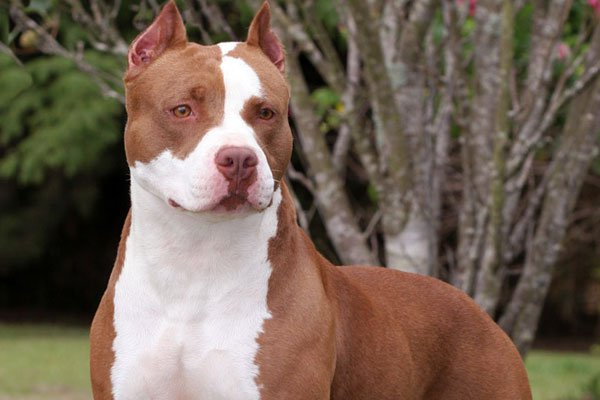
\includegraphics[width=0.5\textwidth]{pitbull.jpg}
    \caption{American Pit Bull Terrier}
    \label{fig:pitbull}
\end{figure}

The design goal of the system is to have a battle system that can both be extremely deadly, where any bite could potentially kill, and also include painfully long-drawn-out matches determined by endurance. It is meant to be a stone-paper-scissors-like system, where a very aggressive dog (like an American Pit Bull Terrier seen in figure \ref{fig:pitbull}) would be able to beat a stronger dog (like the Japanese fighting dog Tosa Inu seen in figure \ref{fig:tosa}), but lose to a more courageous dog (like the Russian shepherd dog Caucasian Ovtcharka often used in dog fighting and seen in figure \ref{fig:ovtcharka}, which is genetically breed to guard a flock of sheep on its own, against a pack of wolves and is hence incredibly brave), but the courageous dog would then lose to the stronger dog. We do not have any knowledge whether this is how these dogs would actually do against eachother in a fight, even if this is something that is wildly discussed on internet fora.\

\blockquote{"You want the truth don’t you? Well here goes. I’m 65 years old and fought dogs against the likes of Don Mayfield, Don Maloney, Walter Komosinski, Pete Sweeney, Earl Tudor, Jack Kelly, Jerry Bean, I could go on but what’s the point? I won my share and lost my share. IF there was a better combat dog than the pit bull, then that’s what the pros would be using. You’re talking about a 175 lb. dog against a 50 lb pit bull. The pit bull stil wins. Why? Because the Russian dog WASN’T bred for combat. I’ve seen pit bulls up against everything available and they still win. Are there exceptions to every rule? Of course. When you match a 175 dog against a 50 lb pitbull, the odds are stacked against the smaller dog. But, pound for pound there is NO dog capable of whipping a pit bull. As a matter of fact, I will put a 50 lb. pit bull up against any 175 lb Russian dog in the world. \

There’s an old saying that goes like this, “it’s not the size of the dog in the fight, but the size of the fight in the dog.” The American Pit Bull is the world’s greatest combat animal ever bred. If you think placing a 175 lb. Russian dog against a 50 lb. pit bull you have my deepest sympathies. When the pit bull grabs the big dog by the now and won’t let go, let’s see how much screaming goes on fro the big dog. And make no mistake, the pit bull IS gonna at some time or another bite the bigger dog in a place he ain’t gonna care much for. And once again, if the “pros” who fight dogs felt like the Russian dog was the best combat dog, don’t you think they’d be using them instead of the lowly pit bull? ‘Nuff said."\

- \textit{American Pitbull Terrier vs Ovcharka?} \url{http://www.russiandog.net/pitbull-terrier-vs-ovcharka.html}
\label{pitbullQuote}}

\begin{figure} 
	\centering
    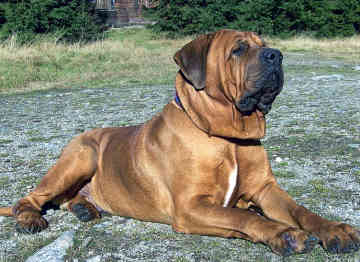
\includegraphics[width=0.5\textwidth]{tosa.jpg}
    \caption{Tosa Inu}
    \label{fig:tosa}
\end{figure}

\begin{figure}
	\centering
    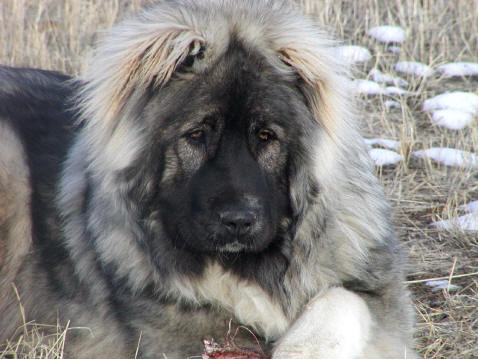
\includegraphics[width=0.5\textwidth]{ovtcharka.jpg}
    \caption{Caucasian Ovtcharka}
    \label{fig:ovtcharka}
\end{figure}

In the prototype the first fight is hard-coded to be a win for the player and the fourth match will always be a loss. So if the \textit{wrong} dog were to kill the other and win, it would instead miss.\

\subsection{Actions Between Fights}
Between the dog fights the players had the option of either training their dogs, breeding the dogs or catching a new dog. As mentioned in \ref{limitations} both catching other dogs or breeding is not possible to succeed in the prototype and are only there to give the illusion of a more expansive game. The training is done by rapidly tapping the screen to get the bar seen in figure \ref{fig:training} full up. Then the dog's respective stat increases by one. If the bar becomes completely empty before this, the training fails and nothing happens.\ 


\begin{figure}[h!] 
	\centering
    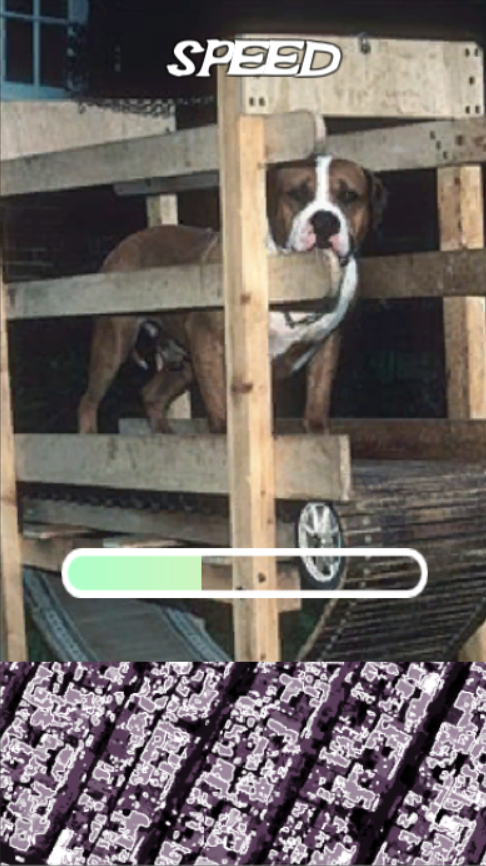
\includegraphics[width=0.5\textwidth]{Training.png}
    \caption{Training screen from the \textit{Rat Kid Dog Fight!} prototype}
    \label{fig:training}
\end{figure}

By only allowing one choice per game week, we implicitly associate a cost with the action, and an investment in your dog. This also frames the game loop nicely, so the main loop becomes Train/Catch/Breed-\>Dog Fight-\>Train/Catch/Breed-\>... \